%%% The main file. It contains definitions of basic parameters and includes all other parts.

% Meta-data of your thesis (please edit)
\input metadata.tex

% Generate metadata in XMP format for use by the pdfx package
\input xmp.tex

%% Settings for single-side (simplex) printing
% Margins: left 40mm, right 25mm, top and bottom 25mm
% (but beware, LaTeX adds 1in implicitly)
% \documentclass[12pt,a4paper]{report}
% \setlength\textwidth{145mm}
% \setlength\textheight{247mm}
% \setlength\oddsidemargin{15mm}
% \setlength\evensidemargin{15mm}
% \setlength\topmargin{0mm}
% \setlength\headsep{0mm}
% \setlength\headheight{0mm}
% \openright makes the following text appear on a right-hand page
% \let\openright=\clearpage

%% Settings for two-sided (duplex) printing
% \documentclass[12pt,a4paper,twoside,openright]{report}
% \setlength\textwidth{145mm}
% \setlength\textheight{247mm}
% \setlength\oddsidemargin{14.2mm}
% \setlength\evensidemargin{0mm}
% \setlength\topmargin{0mm}
% \setlength\headsep{0mm}
% \setlength\headheight{0mm}
% \let\openright=\cleardoublepage

%% If the thesis has no printed version, symmetric margins look better
\documentclass[12pt,a4paper]{report}
\setlength\textwidth{145mm}
\setlength\textheight{247mm}
\setlength\oddsidemargin{10mm}
\setlength\evensidemargin{10mm}
\setlength\topmargin{0mm}
\setlength\headsep{0mm}
\setlength\headheight{0mm}
\let\openright=\clearpage

%% Generate PDF/A-2u
\usepackage[a-2u]{pdfx}

%% Prefer Latin Modern fonts
\usepackage{lmodern}
% If we are not using LuaTeX, we need to set up character encoding:
\usepackage{iftex}
\ifpdftex
\usepackage[utf8]{inputenc}
\usepackage[T1]{fontenc}
\usepackage{textcomp}
\fi

%% Further useful packages (included in most LaTeX distributions)
\usepackage{amsmath}        % extensions for typesetting of math
\usepackage{amsfonts}       % math fonts
\usepackage{amsthm}         % theorems, definitions, etc.
\usepackage{array}          % multicolumns
\usepackage{bm}             % boldface symbols (\bm)
\usepackage{booktabs}       % improved horizontal lines in tables
\usepackage{caption}        % custom captions of floating objects
\usepackage{dcolumn}        % improved alignment of table columns
\usepackage{floatrow}       % custom float environments
\usepackage{graphicx}       % embedding of pictures
\usepackage{indentfirst}    % indent the first paragraph of a chapter
\usepackage[nopatch=item]{microtype}   % micro-typographic refinement
\usepackage{multirow}
\usepackage{paralist}       % improved enumerate and itemize
\usepackage{subcaption}     % support for multiple images within one figure
\usepackage[nottoc]{tocbibind} % makes sure that bibliography and the lists
			    % of figures/tables are included in the table
			    % of contents
\usepackage{xcolor}         % typesetting in color

% The hyperref package for clickable links in PDF and also for storing
% metadata to PDF (including the table of contents).
% Most settings are pre-set by the pdfx package.
\hypersetup{unicode}
\hypersetup{breaklinks=true}

% Packages for computer science theses
\usepackage{algpseudocode}  % part of algorithmicx package
\usepackage{algorithm}
\usepackage{fancyvrb}       % improved verbatim environment
\usepackage{listings}       % pretty-printer of source code

% You might want to use cleveref for references
% \usepackage{cleveref}

% Set up formatting of bibliography (references to literature)
% Details can be adjusted in macros.tex.
%
% BEWARE: Different fields of research and different university departments
% have their own customs regarding bibliography. Consult the bibliography
% format with your supervisor.
%
% The basic format according to the ISO 690 standard with numbered references
\usepackage[natbib,style=iso-numeric,sorting=none]{biblatex}
% ISO 690 with alphanumeric references (abbreviations of authors' names)
%\usepackage[natbib,style=iso-alphabetic]{biblatex}
% ISO 690 with references Author (year)
%\usepackage[natbib,style=iso-authoryear]{biblatex}
%
% Some fields of research prefer a simple format with numbered references
% (sorting=none tells that bibliography should be listed in citation order)
%\usepackage[natbib,style=numeric,sorting=none]{biblatex}
% Numbered references, but [1,2,3,4,5] is compressed to [1-5]
%\usepackage[natbib,style=numeric-comp,sorting=none]{biblatex}
% A simple format with alphanumeric references:
%\usepackage[natbib,style=alphabetic]{biblatex}

% Load the file with bibliography entries
\addbibresource{bibliography.bib}

% Our definitions of macros (see description inside)
\input macros.tex

%%% Title page and various mandatory informational pages
\begin{document}
%%% Title page of the thesis and other mandatory pages

%%% Inscriptions at the opening page of the hard cover

% We usually do not typeset the hard cover, but if you want to do it, change \iffalse to \iftrue
\iffalse

\pagestyle{empty}
\hypersetup{pageanchor=false}
\begin{center}

\large
Charles University

\medskip

Faculty of Mathematics and Physics

\vfill

{\huge\bf\ThesisTypeTitle}

\vfill

{\huge\bf\ThesisTitle\par}

\vfill
\vfill

\hbox to \hsize{\YearSubmitted\hfil \ThesisAuthor}

\end{center}

\newpage\openright
\setcounter{page}{1}

\fi

%%% Title page of the thesis

\pagestyle{empty}
\hypersetup{pageanchor=false}
\begin{center}

\centerline{\mbox{
\includegraphics[width=166mm]{../img/logo-en.pdf}}}

\vspace{-8mm}
\vfill

{\bf\Large\ThesisTypeTitle}

\vfill

{\LARGE\ThesisAuthor}

\vspace{15mm}

{\LARGE\bfseries\ThesisTitle\par}

\vfill

\Department

\vfill

{
\centerline{\vbox{\halign{\hbox to 0.45\hsize{\hfil #}&\hskip 0.5em\parbox[t]{0.45\hsize}{\raggedright #}\cr
Supervisor of the \ThesisTypeName{} thesis:&\Supervisor \cr
\ifx\ThesisType\TypeRig\else
\noalign{\vspace{2mm}}
Study programme:&\StudyProgramme \cr
\fi
}}}}

\vfill

Prague \YearSubmitted

\end{center}

\newpage

%%% A page with a solemn declaration to the thesis

\openright
\hypersetup{pageanchor=true}
\vglue 0pt plus 1fill

\noindent
I declare that I carried out this \ThesisTypeName{} thesis on my own, and only with the cited
sources, literature and other professional sources.
I understand that my work relates to the rights and obligations under the Act No.~121/2000 Sb.,
the Copyright Act, as amended, in particular the fact that the Charles
University has the right to conclude a license agreement on the use of this
work as a school work pursuant to Section 60 subsection 1 of the Copyright~Act.

\vspace{10mm}

\hbox{\hbox to 0.5\hsize{%
In \hbox to 6em{\dotfill} date \hbox to 6em{\dotfill}
\hss}\hbox to 0.5\hsize{\dotfill\quad}}
\smallskip
\hbox{\hbox to 0.5\hsize{}\hbox to 0.5\hsize{\hfil Author's signature\hfil}}

\vspace{20mm}
\newpage

%%% Dedication

\openright

\noindent
\Dedication

\newpage

%%% Mandatory information page of the thesis

\openright
{\InfoPageFont

\vtop to 0.5\vsize{
\setlength\parindent{0mm}
\setlength\parskip{5mm}

Title:
\ThesisTitle

Author:
\ThesisAuthor

\DeptType:
\Department

Supervisor:
\Supervisor, \SupervisorsDepartment

Abstract:
\Abstract

Keywords:
{\def\sep{\unskip, }\ThesisKeywords}

\vfil
}

% In Czech study programmes, it is mandatory to include Czech meta-data:

\ifx\StudyLanguage\LangCS

\vtop to 0.49\vsize{
\setlength\parindent{0mm}
\setlength\parskip{5mm}

Název práce:
\ThesisTitleCS

Autor:
\ThesisAuthor

\DeptTypeCS:
\DepartmentCS

Vedoucí bakalářské práce:
\Supervisor, \SupervisorsDepartmentCS

Abstrakt:
\AbstractCS

Klíčová slova:
{\def\sep{\unskip, }\ThesisKeywordsCS}

\vfil
}

\fi

}

\newpage

%%% Further pages will be numbered
\pagestyle{plain}

%%% A page with automatically generated table of contents of the thesis

\tableofcontents

%%% Each chapter is kept in a separate file
\chapter*{Introduction}
\addcontentsline{toc}{chapter}{Introduction}


\chapter{Problem description}\label{ch:problem}
\section{Input description}

The following instance data define a problem instance.

\begin{itemize}
    \item Set of customer requests $R$, where every request consists of its unique identifier $id$, the earliest time of departure $t_d$ (number of seconds from the start of the simulation), group size (number of passengers in the group), coordinates of the group's departure location, and coordinates of the group's arrival location. The size of any group cannot exceed the capacity of the largest available bus.
    \item The coordinates of the \textit{depot}
    \item The \textit{bus type} available from the depot. The bus type must include the capacity of the bus $c$, the operational cost of the bus per kilometer $o$, and the one-time fee for using the bus $f$.
    \item Distances between each point (in meters).
    \item Travel times between each point (in seconds).
\end{itemize}

\section{Solution} \label{sec:solution}

The solution is a set of routes. Each route is given as a list of group indices in the order the bus handles their pick-ups and drop-offs.

For a solution to be valid, the following constraints must hold.

\begin{enumerate}[(1)]\label{constraints}
    \setlength\itemsep{0pt}
    \item Each group is handled by exactly one bus.
    \item Each group must be picked up and dropped off by a bus exactly once and as a whole.
    \item No bus carries more passengers than its capacity allows it to.
\end{enumerate}

This means that each group can appear in only one route. Each group's index must be included in its corresponding route \textit{exactly twice} - the first occurrence marks the pick-up, and the second occurrence marks the drop-off.

Every route needs to start and end at the depot. Since only one is available, it is implicitly added to every route's beginning and end.

\section{Objective function}
\label{sec:objective}

Since the goal is to minimize the costs, they form the foundation of the function. With $S$ being the solution, $r$ a route within the solution, $r_i$ the $i$th stop on the route, and $d(r_i, r_j)$ the distance between stops $r_i$ and $r_j$ in kilometers, the total operational cost of the buses is given by the equation
\begin{equation}\label{eq:objective_costs}
    \text{operational cost} \equiv \sum_{r \in S} ( f + o \cdot \sum_{i=1}^{|r|}d(r_{i-1},r_{i}))
\end{equation}


We must also account for the group's \textit{delays} when evaluating a solution. The delay for each group is calculated as the difference between the time we drop the group off and the \textit{expected arrival time}, which is defined as the sum of the group's departure time and the travel time between the group’s departure and destination points.

We represent the ``satisfaction'' of the customers by the equation
\begin{equation}\label{eq:objective_satisfaction}
     \text{satisfaction cost} \equiv \sum_{g \in groups} p_t \cdot d_g^2
\end{equation}
where $p_t$ is the penalty constant for late arrival and $d_g$ is the group's delay. The group's delay is squared to penalize larger delays more. The penalty constant is a hyperparameter and depends on the priority of handling all the customers as soon as possible at the expense of higher operational costs.

The objective function is then the sum of the \textit{operational} and \textit{satisfaction} cost.

\begin{equation}\label{eq:objective}
    \sum_{r \in S} ( f + o \cdot \sum_{i=1}^{|r|}d(r_{i-1},r_{i})) + \sum_{g \in groups} p_t \cdot d_g^2
\end{equation}

\section{Input data generation}

We create our own benchmark data to compare the algorithms presented in the thesis. We have two basic dataset types, \textit{uniformly distributed} and \textit{commute}.

Given an OpenStreetMaps area, the number of requests to generate, the maximum size of a group in a request, and the latest possible departure time of a group, the \textit{uniformly distributed} generator creates requests where departure and destination coordinates are a randomly chosen public transport platform in the given area. The departure times and group sizes are chosen randomly. The number of platforms to sample from can be limited to force multiple customers to use the same platform for departure/destination. The depot is also randomly chosen from the available platforms, and the available bus type's \textit{capacity}, \textit{operational cost per km}, and \textit{fixed cost for usage} is given as a parameter.

The \textit{commute} generator generates requests similarly to the \textit{uniformly distributed generator} but takes three OpenStreetMaps areas instead, an \textit{area from}, \textit{area to}, and a \textit{depot area}. The departure coordinates are randomly chosen platforms from \textit{area from}, and destination coordinates are randomly chosen platforms from \textit{area to}. The depot coordinates are randomly chosen from the platforms in the \textit{depot area}. We can also use a \textit{two-way} parameter, which makes the generator also generate requests from \textit{area to} to \textit{area from}. The departure times for both directions are still randomly generated based on the latest possible departure time.

The customer requests are stored in \textit{GeoJSON} file, whose structure is described in detail in the attached \textit{JSON schema}.

We must also generate the \textit{distance} and \textit{duration} matrices. We use the Open Source Routing Machine (\textit{OSRM}) API \cite{luxen-vetter-2011}, which has a \textit{table service} that can generate both matrices based on a list of coordinates. The matrices are stored in separate \textit{CSV} files.

\iffalse

\section{Stuff to sort}

\begin{itemize}
    \item Since \textit{DARP} is a real-world problem, we will make some simplifications to the problem to simplify the problem's simulation. We won't constrain or penalize route lengths (we can assume that the buses can refill fuel between stops with no time penalty). We will also mostly ignore most of the needs of the bus driver, such as compulsory time breaks after driving for a certain amount of time or having limited working hours. \xxx{Probably move to the introduction}
\end{itemize}

\fi
\chapter{Genetic algorithm}\label{ch:genetic}

The concept of genetic algorithms to solve computationally hard problems was first presented by John Holland \cite{Holland:1992}. Starting with a \textit{population} formed with initial (in most cases random) solutions (called \textit{individuals}), \textit{crossover} and \textit{mutation} operators are applied to gradually improve the fitness score of the population and thus find the best individual overall.

The most essential thing when designing a specific genetic algorithm is the encoding of an individual. Based on the encoding, we need to choose the genetic operators - \textit{crossover} and \textit{mutation}. The \textit{crossover} operator takes two random individuals (\textit{parents}) from the population and uses them to create two new individuals, which combine the properties of the parents. The \textit{mutation} operator takes only one individual and makes a change within him. The change should usually be small and can be either completely random or try to improve the individual using some heuristic (called a \textit{smart mutation}). The operators are performed on an individual or pair of individuals with a given probability (so in each generation, only some individuals participate in crossover or are mutated).

After the operators are applied, the new population is created using the \textit{selection}. In our cases, the selection can either be a \textit{roulette wheel selection} or a \textit{tournament selection}. In the \textit{roulette wheel selection}, we randomly sample individuals from the current population, but the individuals are weighted using their fitness value. When using the \textit{tournament selection}, we take $t$ (usually 2 or 3) random individuals from the population and compare their fitness values. The best one is chosen and added to the new population. This process is repeated until the new population is fully populated.

Apart from using the \textit{roulette wheel} or \textit{tournament} selection, we employ a strategy called \textit{elitism}. After the new population is sampled, we choose $n$ individuals randomly and replace them with the first $n$ best individuals from the old population. This ensures that the best individual in each population survives into the next generation.

\hspace{0pt}

We present three different encodings of an individual:

\begin{itemize}
    \item Individual as routes made of stops (EVO-STOPS)
    \item Individual as separate clustering and routing (EVO-CR)
    \item Individual as only clustering, with routing solved with greedy heuristic (EVO-H)
\end{itemize}

Each encoding has its separate population initialization and genetic operators, described in detail in sections \ref{sec:evo-stops} to \ref{sec:evoh}. They share the fitness function, which is evaluated by transforming the individual into a solution and evaluating the objective function defined in \ref{eq:objective}.

\section{Individual as routes of stops}\label{sec:evo-stops}

\subsection{Coding of an individual}

The individual is encoded as a list of routes, where each route is a \textbf{list of stops} in the order the bus visits them.

Transforming the individual into a solution is done by simulation.  We simulate every route - at each stop, we pick up any group waiting for the bus at that stop and drop off every group present on the bus that can be dropped off. If multiple groups are waiting at the stop, but not all can fit into the bus, we prioritize the groups that are waiting longer. At the end of the route, if any groups are left on the bus, we drop them off in the order of their departure time and return to the depot. \label{evostops-catchroute}After all route simulations are completed, we create another route by taking all the groups not picked up by any bus, picking them up, and immediately dropping them off in the order of their departure time. This ensures that the simulation returns a valid solution.

The difference between the encoding of a solution and our individual is that the individual uses stops instead of groups to encode a route. The main reason for introducing this change was that maintaining the correctness of the solution after performing the genetic operators on it would be problematic. Making a (semi-)random change in the individual could easily end up in the violation of constraints \hyperref[constraints]{(2)} or \hyperref[constraints]{(3)}. Using stops instead of groups eliminates the problem of invalidating an individual since there is no invalid individual.

\subsection{Initial population}

We present two ways to create the initial population - \textit{random} and \textit{greedy}.

The \textit{random} individual generator generates random sequences of stops and takes as a parameter the number of buses to use and the maximum allowed length of a route.

The \textit{greedy} generator tries to generate already feasible routes. At each stop, we generate a set of reasonable next actions - picking up a new group or dropping off a group present on the bus. When considering groups to pick up, we only consider those whose departure time is close to the arrival time to their pick-up stop. For this, the generator takes a parameter defining how large this \textit{time window} should be. If no more options exist, the bus ends the route by traveling to the depot. The generator can also be limited by parameters that define the maximum number of buses that can be used or the maximum number of groups that can be picked up within one route.

\subsection{Genetic operators}

\subsubsection{Crossover}

We use a simple \textit{one-point crossover}. We take \textbf{one} random route from each individual, select a \textit{crossover point}, and swap the right parts of the routes between the individuals.

We decided to use the crossover on only one of the routes for each individual. This is because even a change in one route is usually quite a big change - it can easily result in not picking up or dropping off some groups and, therefore, making the new individual largely penalized. However, it also makes the genetic algorithm much more exploratory.

\subsubsection{Mutation}

Unlike crossover, we have many options on what mutation operators to choose. We decided to implement many of them as \textit{``submutations''} and randomly choose one at each mutation. The probability of each \textit{``submutation''} is determined by its weight, and the weights are set before an experiment as hyper-parameters.

The possible \textit{``submutations''} are:
\begin{itemize}
    \setlength\itemsep{0pt}
    \item Delete a random stop from a randomly chosen route.
    \item Add a random stop to a randomly chosen route.
    \item Change a stop to a random one in a randomly chosen route.
    \item Reverse a random sub-route of a randomly chosen route. This is the main source of changing the stops' order.
    \item Shuffle the routes within the solution. This can greatly impact the simulation when evaluating the fitness function since each group is picked up by the first bus (in the simulation order) that arrives at their stop at the right time. If more buses travel through the same stop, groups on that stop can be picked up by a completely different bus.
    \item ``Smart mutation'' - depending on the quality of the individual, it either tries to add an ``unhandled'' group to a random route, or it tries to perform a swap of a group between 2 routes. In both cases, we need to insert to a route both pick-up and drop-off points. The maximum distance between these points is given as a parameter.
\end{itemize}

\section{Individual as separate clustering and routing}\label{sec:evocr}

\subsection{Coding of an individual}

The individual consists of two parts: the mapping between a group and a route, which \textit{clusters} the groups, and the order in which the groups are picked up and dropped off.

The mapping is defined by an array, where the array indices represent the \textit{group identifiers} and the values represent the \textit{identifier of the route that handles the group}. The maximum number of routes is given as a parameter to limit the number of routes used.

The order of pick-ups and drop-offs is defined by an array, where every group occurs twice; the first occurrence marks the pick-up, and the second marks the drop-off.

To transform an individual into a solution, for each route, we first determine which groups are handled by that route, and then we construct the route by picking the group's indices in the order they are present in the individual's order-defining array. When constructing a route, if the capacity constraint would be violated by picking up the next group, we drop off groups with the earliest departure times until the bus has enough capacity to pick up the group.

\subsection{Initial population}

We generate the initial solutions randomly - given the maximum number of routes, we assign each group to a random route, and the order of the groups is created by a random shuffle.

\subsection{Genetic operators}

\subsubsection{Crossover}

In the crossover, we only cross the order of handling the groups. We first transform the order array into a permutation by adding $|R|$ to every second occurrence of each group. On this permutation, we use the \textit{Partially Mapped Crossover (PMX)} \cite{Goldberg1985AllelesLA}. We then transform the permutation back to the order array by subtracting $|R|$ from every second occurrence of each group.

\subsubsection{Mutation}

Mutation has multiple options for changing the individual. It can change the route assignment by either swapping two random groups between routes or assigning a random route to a random group, or it can change the order by either reversing a part of the order array or swapping two values in the order array.

\section{Individual as only clustering with heuristic routing}\label{sec:evoh}

\subsection{Coding of an individual}

The individual comprises only the mapping between the groups and the routes, which is stored in an array, where the array indices represent the group identifiers and the values represent the identifier of the route that handles the group.

To convert an individual into a solution, we first divide the groups into routes based on the individual. The order in which we handle the groups within a route is then calculated based on a greedy space-time nearest neighbor heuristic described by Baugh et al. \cite{Baugh1998INTRACTABILITYOT}.

The heuristic is based on assigning a \textit{cost} to each movement, which is calculated as a weighted sum of the travel time between the stops and the
\textit{time violation}. For pick-up nodes, the \textit{time violation} is the amount of time either the bus had to wait for the group or the group had to wait for the bus. For drop-off nodes, it is equal to the delay of the dropped-off group.

When evaluating the route, we first find $d$ ``cheapest'' possible options to travel to, where $d$ is a heuristic depth parameter. We only choose those options that would not violate any constraints defined in the section \ref{sec:solution}. For each of the options, we then try to determine the cost of the resulting route if we choose this option. We do this by evaluating the cost of a route where, for $d$ stops, we would always choose the ``cheapest'' available option. Based on the costs of these routes, we then choose the best option overall. We then repeat this process until no options are available and all groups are picked up and dropped off.

\begin{algorithm}
\caption{Move cost between nodes i and j}
\label{alg:evoh_move_cost}
\begin{algorithmic}
\Require $i, j, current\_time$
\State $travel\_time \gets durations[i, j]$
\State $arrival\_time \gets current\_time + travel\_time$
\If{$j$ is a pick-up node}
    \State $expected\_time \gets Group(j).departure\_time$
\Else
    \State $group\_duration \gets durations[Group(j).start, Group(j).end]$
    \State $expected\_time \gets Group(j).departure\_time + group\_duration$
\EndIf
\State $tw\_viol \gets |arrival\_time - expected\_time|$
\State \textbf{return} $w_{travel\_time} \cdot travel\_time + w_{time\_window} \cdot tw\_viol$
\end{algorithmic}
\end{algorithm}

\subsection{Initial population}

We generate the initial solutions randomly - given the maximum number of routes to use, we assign each group to a random route.

\subsection{Genetic operators}

\subsubsection{Crossover}

We use a uniform crossover - for each of the two individuals, we go through the group-routes assignment, and with a given probability, we change the current assignment to the one in the second individual.

\subsubsection{Mutation}

The mutation swaps two random groups between their routes or assigns a random route to a random group.

\section{Hyperparameters}\label{sec:genetic_hyperparams}

\subsection{Individual as routes of stops}

The hyper-parameter values largely influence the behavior of the algorithm. We perform a series of experimental measurements to find the best values for the final experiments.

\begin{figure}[b]
    \centering
    \begin{subfigure}[b]{0.45\textwidth}
        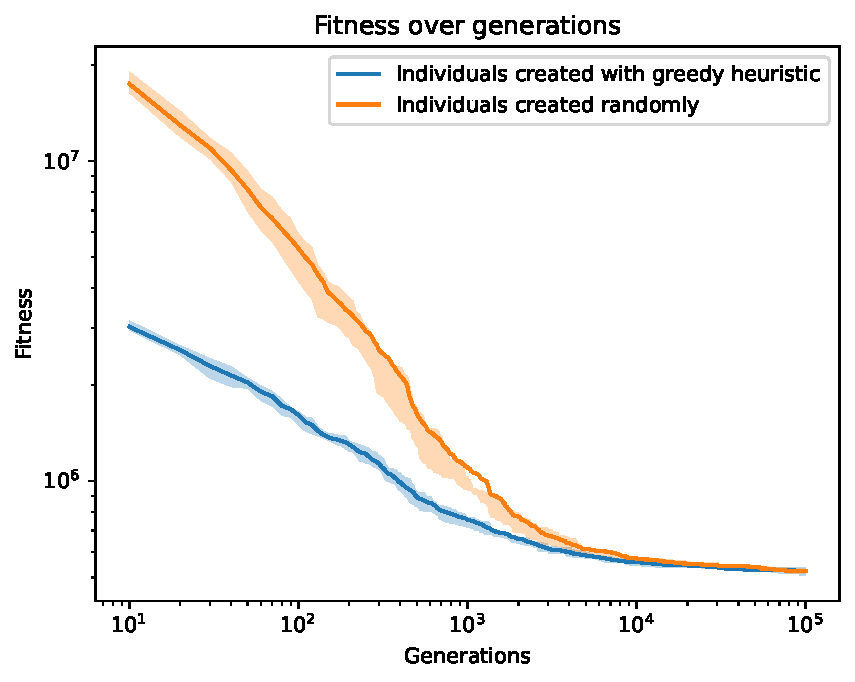
\includegraphics[width=\textwidth]{img/evo1_create_ind_random.pdf}
        \caption{Randomly distributed data}
        \label{fig:evo1_cind_random}
    \end{subfigure}
    \begin{subfigure}[b]{0.45\textwidth}
        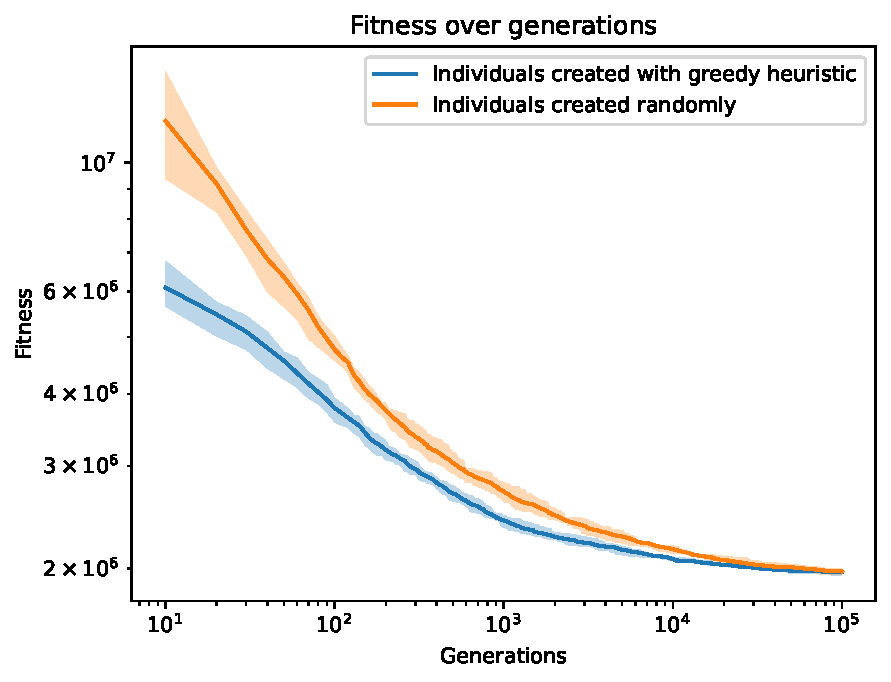
\includegraphics[width=\textwidth]{img/evo1_create_ind_commute.pdf}
        \caption{Long distance commute data}
        \label{fig:evo1_cind_commute}
    \end{subfigure}
    \caption{Individual as stops - population initialization}
    \label{fig:evo1_create_ind}
\end{figure}

\label{experiment_graph_description}
We will describe the experiments on the population initialization function. For both dataset types, we conduct two experiments, one with \textit{greedy} initialization and one with \textit{random} initialization. Both datasets are made of 50 customer requests, with group sizes between 1 and 10 persons and departure times in a 2-hour window. Each experiment runs the genetic algorithm 10 times. In figure \ref{fig:evo1_create_ind}, for each experiment, the mean fitness of the 10 runs is depicted as the primary line, accompanied by the first and third quartiles represented as a translucent region. Both $x$ and $y$ axes are logarithmic.

From the figure, we can see that for both datasets, the \textit{greedy} initialization resulted in faster convergence at the beginning. We therefore decided to use the \textit{greedy} initialization.

The rest of the hyper-parameter values were chosen similarly and are shown in the table \ref{tab:evo_stops_hyperparams}.

\begin{table}[ht]
    \centering
    \begin{tabular}{lc}
        Mutation probability & 0.8 \\
        Crossover probability & 0.2 \\
        Selection & tournament ($t=2$) \\
        Population size & 40 \\
        Create individual function & greedy \\
        Smart mutation weight & 12 \\
        Reverse a route weight & 3 \\
        Add/Delete/Change a stop randomly weight & 9 \\
        Shuffle individual weight & 2 \\
        Smart mutation maximum pick-up-drop-off distance & 20 \\
    \end{tabular}
    \caption{Individual as stops - hyper-parameter settings}
    \label{tab:evo_stops_hyperparams}
\end{table}

\subsection{Individual as separate clustering and routing}

The hyper-parameter settings for both dataset types were chosen experimentally and are shown in the table \ref{tab:evo_cr_hyperparams}.

\begin{table}[ht]
    \centering
    \begin{tabular}{lc}
        Mutation probability & 0.8 \\
        Crossover probability & 0.4 \\
        Selection & tournament ($t=2$) \\
        Population size & 30 \\
        Mutate route assignments probability & 0.5 \\
        Swap two groups between routes mutation probability & 0.5 \\
        Reverse a part of the order array mutation probability & 0.7 \\ 
    \end{tabular}
    \caption{Individual as cluster and route - hyper-parameter settings}
    \label{tab:evo_cr_hyperparams}
\end{table}

\subsection{Individual as only clustering with heuristic routing}

The hyper-parameter settings for both dataset types were chosen experimentally and are shown in the table \ref{tab:evo_ch_hyperparams}.

\begin{table}[ht]
    \centering
    \begin{tabular}{lc}
        Mutation probability & 0.8 \\
        Crossover probability & 0.3 \\
        Selection & tournament ($t=3$) \\
        Population size & 20 \\
        Travel time weight in heuristic cost & 1 \\
        Time window violation weight in heuristic cost & 2 \\
        Uniform crossover switch assignment probability & 0.2 \\
        Swap two groups between routes mutation probability & 0.5 \\
    \end{tabular}
    \caption{Individual as only clustering with heuristic routing - hyper-parameter settings}
    \label{tab:evo_ch_hyperparams}
\end{table}

\chapter{Ant Colony Optimization}

The \textit{Ant Colony Optimization (ACO)} algorithm is a probabilistic optimization metaheuristic first presented by Dorigo and Stützle \cite{Dorigo2010}. The algorithm is based on the behavior of ants. When searching for food, multiple ants scatter around their anthill. They lay down small amounts of pheromone to remember the way back. If their search is successful, they return to the anthill while laying down a much stronger layer of pheromone to mark the path to the finding. Other ants can then follow this pheromone trail instead of searching randomly. The pheromone, however, slowly evaporates, so the trail gets thinner for longer paths. This allows the ants to find the shortest paths to nearby food.

The \textit{ACO} builds on this metaphor. Our \textit{ants} generate possible solutions by moving through the \textit{parameter space}. When they create a solution, they update the \textit{pheromone} stored in the \textit{pheromone matrix} based on the fitness value of their solution. When new ants then move through the parameter space, they follow paths with higher pheromone levels, increasing the chance of finding a better solution. Apart from the pheromone levels, the ant also decides on the heuristic value of the path - \textit{attractiveness}.

We represent our \textit{parameter space} as an oriented graph. Vertices are the group's pick-ups and drop-offs. Edges represent the traveling, e.g., the edge between the group’s $i$ drop-off and the group’s $j$ pick-up represents the path between the group’s $i$ destination point and the group’s $j$ departure point. We must also add a node for the depot. The solution is then a set of paths through the graph, where each path satisfies the constraints defined in \ref{constraints}.

\section{Creating solutions}

An \textit{ant} generates new routes until all the customer requests are handled. Each route starts by picking up the first unhandled group with the lowest departure time. We then create a set of all possible options: pick up a new group, drop off a group sitting in the bus, and, only if the bus is empty, return to the depot. The probability of picking each option is based on the amount of pheromone between the two nodes $\tau$ and the attractiveness value of the transition $\nu$. The probability of transition from vertex $i$ to vertex $j$ is then proportional to $\tau_{ij}^\alpha \cdot \nu_{ij}^\beta$, where $\alpha$ and $\beta$ are hyperparameters specifying the ratio between $\tau$ and $\nu$. If the option to return to the depot is selected, the route ends.

\subsubsection{Attractiveness}

We use a simplified heuristic used in section \ref{sec:evoh}. The attractiveness is equal to a weighted sum of the travel time between the stops and the time window violation - how soon or late would the bus arrive.

When considering dropping off a group, we can adjust the attractiveness by multiplying it with a \textit{drop-off attractiveness bonus} hyperparameter. Setting it high can force the ants to drop off groups as soon as possible to minimize delays while setting it low helps fill the bus's capacity, which can sometimes minimize travel times. We define this coefficient as a function taking the current route and the \textit{ant's id}. The \textit{ant's id} parameter can be useful for assigning different strategies to different ants, and passing the route allows one to make decisions based on its length.

When calculating attractiveness for returning to the depot, we have no time window to consider in the weighted sum. Instead, we only multiply the travel time to the depot with the \textit{depot attractiveness coefficient} hyperparameter to favor or disfavor the depot and, therefore, end the current route. This coefficient is also defined as a function taking the current route.

\section{Pheromones}

The pheromone matrix is of size $(2|G| + 1) \times (2|G| + 1)$, where $G$ is the set of all groups. For each group with id $i$, the pheromone at index $i$ represents the probability of the group being picked up, and the pheromone at index $i + |G|$ represents the likelihood of the group being dropped off. The last index represents the depot. We initialize it at the beginning of the algorithm uniformly.

After all the ants generate their solutions, we need to update the pheromone matrix. Firstly, we \textit{evaporate} the current pheromone by setting the matrix to $\tau = (1 - \rho)\tau$, where $\rho$ is a hyperparameter. Then, we update the pheromones based on the generated solutions and their fitness values. The update is defined as $\Delta\tau_{ij} = \sum_{k=1}^{ants}\Delta\tau_{ij}^{k}$, where
\begin{equation}
    \Delta\tau_{ij}^{k} = 
        \begin{cases}
        Q / L_k & \text{if edge $ij$ was used in the $k$th solution} \\
        0 & \text{otherwise}
        \end{cases}
\end{equation},
$Q$ is a hyperparameter and $L_k$ is the fitness value of the $k$th solution.

After updating the pheromone matrix, we start a new iteration by generating new solutions for each ant. This is done until the iteration limit is reached or until the algorithm stops converging (all ants are generating the exact same solution for many iterations).

\section{Hyperparameters}\label{sec:aco_hyperparams}

The hyper-parameter settings for both dataset types were chosen experimentally and are shown in the table \ref{tab:aco_hyperparams}. 

The experiments were done the same way as in the section \ref{sec:genetic_hyperparams}. For example, in figure \ref{fig:aco_alpha_beta}, we show experiments for setting the $\alpha$ and $\beta$ parameters. We can see that using higher $\alpha = 2$ (or higher) leads to converging to non-optimal solutions. On the \textit{random} dataset, after about 1000 iterations, the algorithm converged to a local optimum and the generated solutions were all the same, so the runs terminated prematurely.

For the random dataset, we set the \textit{drop-off attractiveness bonus} as $50.0$ to motivate dropping the customers off as soon as possible to reduce their delays. For the commute dataset, we set it based on the route's current length - if the route is shorter than a random number between 3 and 5, we set it as $0.1$ to prefer picking up another group. If it is longer, we set it as $100.0$. As a result, the solution contains routes where each bus picks between 3 to 5 groups in the first area and then drops them all off in the destination area. Values 3 and 5 were chosen experimentally, and they depend mostly on the distance between the departure and destination areas and the density of requests in time.

We do not use the \textit{ant\_id} parameter in \textit{drop-off attractiveness bonus} for the final experiments since we failed to find a combination of strategies that would work better than the single strategy used. For example, combining the strategy used for the random dataset with the current one results in finding a local optimum, where the number of buses is close to the number of requests and each bus handles only at most 2 requests.

For the commute dataset, the value of the \textit{depot attractiveness coefficient} does not have much impact on the results - after dropping off all the groups in the destination area, the attractiveness of picking up any group in the source area is too low because the group would be picked up too late, while the depot attractiveness stays high. However, for the random dataset, a lower value, such as $0.1$, lowers the number of buses used. This can be because we only consider returning to the depot when the bus is empty, but we do not penalize the waiting of an empty bus. The attractiveness function, however, still considers the time window violation, so if the bus were to wait for a long time, it would rather return to the depot. While we still need to account for the time windows since picking up groups with earlier departure times might be more favorable, we do not want their attractiveness to be significantly lower than the depot's attractiveness, which does not have a time window. Therefore, lowering the depot attractiveness by multiplying it with a small fixed constant works well.

\begin{figure}
    \centering
    \begin{subfigure}[b]{0.45\textwidth}
        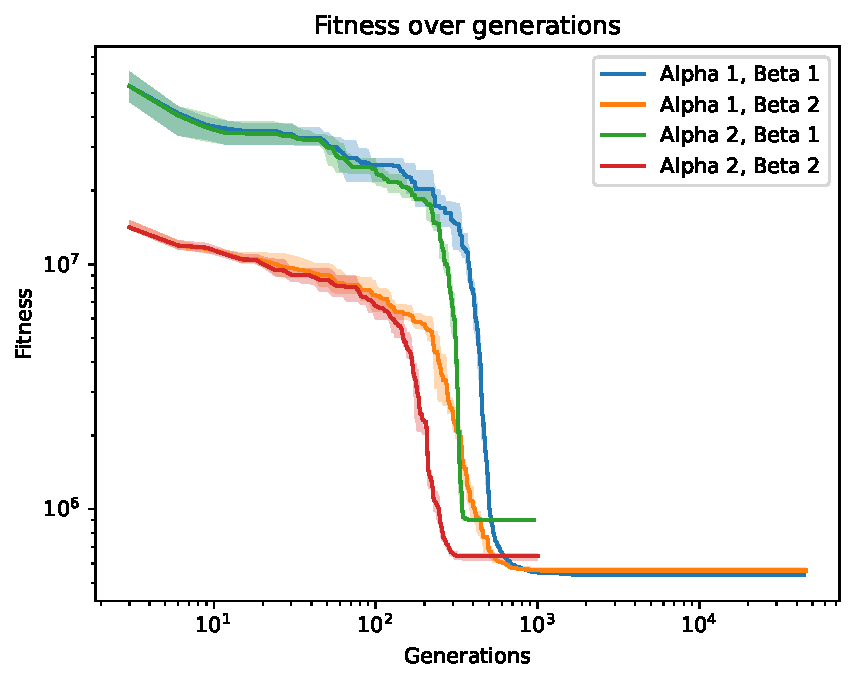
\includegraphics[width=\textwidth]{img/aco_random_ab.pdf}
        \caption{Randomly distributed data}
        \label{fig:aco_ab_random}
    \end{subfigure}
    \begin{subfigure}[b]{0.45\textwidth}
        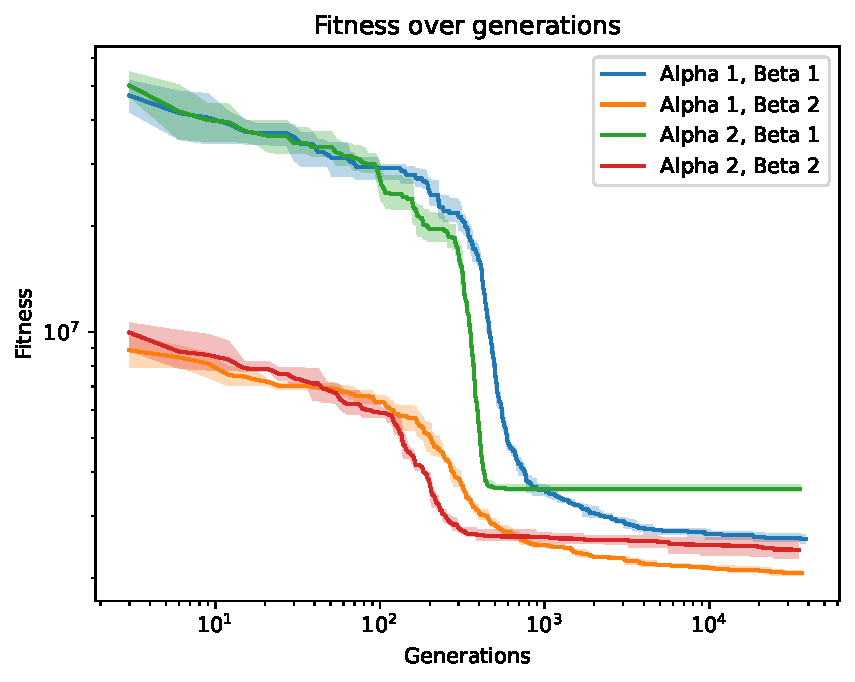
\includegraphics[width=\textwidth]{img/aco_commute_ab.pdf}
        \caption{Long distance commute data}
        \label{fig:aco_ab_commute}
    \end{subfigure}
    \caption{Ant Colony Optimization - Alpha and Beta setting}
    \label{fig:aco_alpha_beta}
\end{figure}

\begin{table}
    \centering
    \begin{tabular}{lcc}
         & Random & Commute \\
        \hline
        $\alpha$ & \multicolumn{2}{c}{1} \\
        $\beta$ & 1 & 2 \\
        $\rho$ & \multicolumn{2}{c}{0.01} \\
        $Q$ & \multicolumn{2}{c}{10 000} \\
        Travel time weight in heuristic cost & 1 & 2 \\
        Time window violation weight in heuristic cost & 2 & 1 \\
        Time window size & 0.01 & 0.1 \\
        Depot attractiveness coefficient & \multicolumn{2}{c}{0.1}
    \end{tabular}
    \caption{Ant Colony Optimization - hyper-parameter settings}
    \label{tab:aco_hyperparams}
\end{table}
\chapter{Experimental results}

To compare the four presented approaches, we generated benchmark datasets and ran all the algorithms on them. In this chapter, we present the results.

\section{Commute dataset}

The used dataset contains 100 passenger requests. Each customer group departs from a random location in Pilsen and travels to a random location in Prague. The distance between the two cities is approximately 90 kilometers. The departure times are randomly distributed in a four-hour time window. Each group is between 1 and 10 people. The depot is set in Prague. It is important to note that the first group in each route gets always picked up on time. This means that the location of the depot has no effect on the group's delays; setting it far from the departure area does, however, make using more buses more costly. The available bus type can take up to 80 persons, its operating cost per kilometer is $80$, and its fixed cost for rental is $50000$.

All the algorithms use the same fitness function, with the delay penalty constant equaling $0.01$.

All the genetic algorithms have a population size set to $30$ individuals, with $3$ best individuals (\textit{elites}) passed from the old to the new population. All the encodings also require an upper limit to the number of buses used, which we set to $30$ buses. The \textit{ACO} uses \textit{20} ants, meaning that 20 new solutions are generated in each iteration. Other parameters are set as described in sections \ref{sec:genetic_hyperparams} and \ref{sec:aco_hyperparams}.

The algorithms ran for exactly 80 minutes, after which they were terminated. Figure \ref{fig:exp_commute} shows the progression of the best fitness value found by each approach. The experiments were repeated 10 times. The value shown is the mean fitness of the 10 runs, with the first and third quartiles depicted by the translucent region. The figure shows progression in time and has both the x and y axis on a logarithmic scale.

\begin{figure}[b]
    \centering
    \includegraphics
    {img/exp_commute_100_time.pdf}
    \caption{Commute dataset - fitness values in time}
    \label{fig:exp_commute}
\end{figure}

Table \ref{tab:exp_commute_route_stats} shows the basic information about the best solution returned by each algorithm - how much all the routes cost, how many kilometers were traveled in total, and how many buses were used. 

\begin{table}
    \centering
    \begin{tabular}{lcccccc}
         & Total costs & Km traveled & Buses used \\
         \hline
         EVO-STOPS & 2231202.82 & 9140.035 & 30 \\
         EVO-CR & \textbf{2153207.33} & 8790.092 & \textbf{29} \\
         EVO-H & 2160139.18 & 8876.740 & \textbf{29} \\
         ACO & 2164447.95 & \textbf{7680.599} & 31 \\
    \end{tabular}
    \caption{Commute dataset - Route statistics}
    \label{tab:exp_commute_route_stats}
\end{table}

Table \ref{tab:exp_commute_delay_stats} shows the statistics about the group's delays - the delay of the most delayed group and the average and median delay of all the groups.

\begin{table}
    \centering
    \begin{tabular}{lcccccc}
         &  Maximum delay & Average delay & Median delay \\
         \hline
         EVO-STOPS & 1963.7 & 658.1 & 672.2 \\
         EVO-CR & 1682.4 & 601.4 & \textbf{590.6} \\
         EVO-H & \textbf{1553.4} & \textbf{595.1} & 596.5 \\
         ACO & 5207.0 & 1537.0 & 1380.9 \\
    \end{tabular}
    \caption{Commute dataset - Delay statistics}
    \label{tab:exp_commute_delay_stats}
\end{table}

When examining the results, we see that no approach is strictly better than all the others. While the Ant Colony Optimization managed to find the shortest set of routes, it failed to deliver the groups in time, with four groups arriving at their destination more than an hour later than if they took a car or a taxi. The \textit{EVO-STOPS} approach returned the solution with the highest total costs and otherwise mediocre results. The \textit{EVO-CR} and \textit{EVO-H} approaches returned very similar results on all fronts.

\chapter*{Conclusion}
\addcontentsline{toc}{chapter}{Conclusion}


%%% Bibliography
%%% Bibliography (literature used as a source)
%%%
%%% We employ bibTeX to construct the bibliography. It processes
%%% citations in the text (e.g., the \cite{...} macro) and looks up
%%% relevant entries in the bibliography.bib file.
%%%
%%% The \bibliographystyle command selects, which style will be used
%%% for references from the text. The argument in curly brackets is
%%% the name of the corresponding style file (*.bst). Both styles
%%% mentioned in this template are included in LaTeX distributions.

\bibliographystyle{plainnat}    %% Author (year)
% \bibliographystyle{unsrt}     %% [number]

\renewcommand{\bibname}{Bibliography}

%%% Generate the bibliography. Beware that if you cited no works,
%%% the empty list will be omitted completely.

\bibliography{bibliography}

%%% If case you prefer to write the bibliography manually (without bibTeX),
%%% you can use the following. Please follow the ISO 690 standard and
%%% citation conventions of your field of research.

% \begin{thebibliography}{99}
%
% \bibitem{lamport94}
%   {\sc Lamport,} Leslie.
%   \emph{\LaTeX: A Document Preparation System}.
%   2nd edition.
%   Massachusetts: Addison Wesley, 1994.
%   ISBN 0-201-52983-1.
%
% \end{thebibliography}


%%% Figures used in the thesis (consider if this is needed)
% \listoffigures

%%% Tables used in the thesis (consider if this is needed)
%%% In mathematical theses, it could be better to move the list of tables to the beginning of the thesis.
% \listoftables

%%% Abbreviations used in the thesis, if any, including their explanation
%%% In mathematical theses, it could be better to move the list of abbreviations to the beginning of the thesis.
\chapwithtoc{List of Abbreviations}
\begin{itemize}
    \item \textbf{DARP} - Dial-A-Ride Problem
    \item \textbf{OSRM} - Open Source Routing Machine
    \item \textbf{EVO-STOPS} - Genetic algorithm implementation where the individual is encoded as a list of routes of stops
    \item \textbf{EVO-CR} - Genetic algorithm implementation where the individual is encoded as separate clustering and routing
    \item \textbf{EVO-H} - Genetic algorithm implementation where the individual represents only clustering and routing is done heuristically
    \item \textbf{ACO} - Ant Colony Optimization
\end{itemize}

%%% Doctoral theses must contain a list of author's publications
\ifx\ThesisType\TypePhD
\chapwithtoc{List of Publications}
\fi

%%% Attachments to the thesis, if any. Each attachment must be referred to
%%% at least once from the text of the thesis. Attachments are numbered.
%%%
%%% The printed version should preferably contain attachments, which can be
%%% read (additional tables and charts, supplementary text, examples of
%%% program output, etc.). The electronic version is more suited for attachments
%%% which will likely be used in an electronic form rather than read (program
%%% source code, data files, interactive charts, etc.). Electronic attachments
%%% should be uploaded to SIS. Allowed file formats are specified in provision
%%% of the rector no. 72/2017. Exceptions can be approved by faculty's coordinator.
\appendix

\chapter{User Guide}

This section contains information needed to run the optimization.

The software is divided into 3 separate parts:

\begin{itemize}
    \setlength\itemsep{0pt}
    \item Data generation
    \item Optimization algorithms
    \item Results evaluation
\end{itemize}

\section{Prerequisites}

For the \textit{data generation} and \textit{results evaluation} modules, the user needs
\begin{itemize}
    \setlength\itemsep{0pt}
    \item a Python interpreter in version 3.11.9. Compatibility with different versions is not guaranteed. Libraries needed and their versions are listed in the \textit{requirements.txt} file. 
    \item a running instance Open Source Routing Machine (OSRM) \cite{luxen-vetter-2011} service. The authors provide a demo server at \texttt{https://router.project-osrm.org}. If you want to host your own, the detailed steps on how to run the service are described in the project's repository \footnote{\url{https://github.com/Project-OSRM/osrm-backend}}. When generating the instance data in some given area, ensure the corresponding OpenStreetMaps extract is available for the OSRM service.
\end{itemize}

The \textit{optimization modules} requires a Julia programming language compiler. The program was tested on Julia versions 1.7.0 and 1.8.5. The packages needed are listed in the \textit{Project.toml} file. The correct environment should be installed by running Julia with the \texttt{--project} argument.

\section{Generating New Instance Data}

The Data used for running this thesis's experiments are available in the attachments. If you want to generate new data, two scripts are available: \textit{dataGeneratorRandom.py} and \textit{dataGeneratorCommute.py}. Both scripts can be configured using command line arguments, described in detail when running the script with \textit{--help}. Running the script generates a new folder with all the needed files: the \textit{GeoJSON} file with customer requests, \textit{CSV} file with the distance matrix, \textit{CSV} file with the duration matrix and a \textit{parameters.txt} file, where the settings of the generator are stored.

The script assumes that the \textit{OSRM} service runs on your local machine. If your instance runs elsewhere, you can override this with the \texttt{--osrm\_url} option, e.g.

\begin{lstlisting}[language=bash, breaklines=true]
    python dataGeneratorCommute.py --osrm_url https://router.project-osrm.org
\end{lstlisting}

\section{Running the optimization algorithms}

All the Julia source files are stored in the \textit{project} folder. Running the algorithms is done by the \textit{runner.jl} script. All the hyper-parameters and other algorithm configurations are stored in the \textit{config.jl} file together with their descriptions.

The easiest way to run the program is with the following command:
\begin{lstlisting}[language=bash]
    julia runner.jl
\end{lstlisting}

The command compiles the program, loads the configuration from \textit{config.jl} and runs the optimization. If you want to override some configuration variables directly from the command line, you can enter key-value pairs \textit{variable=value} in the command. Some of the examples include:

\begin{lstlisting}[language=bash, breaklines=true]
    julia runner.jl algorithm=evolution_stops cross_prob=0.5 mut_prob=0.8 num_generations=20000
\end{lstlisting}

\begin{lstlisting}[language=bash, breaklines=true]
    julia runner.jl input_data_folder_path=my_data algorithm=aco number_of_runs=10 num_ants=10 num_iterations=10000
\end{lstlisting}

When the optimization finishes (by reaching maximum iterations or by exceeding the wall time), the runner stores in an output folder the following files:

\begin{itemize}
    \setlength\itemsep{0pt}
    \item \textit{best\_solution.csv} with the overall best solution found.
    \item \textit{config.yaml} with all the hyperparameter settings for the current run
    \item \textit{run\_$i$.fits}, where $i$ is the run's id for each run, logging the current iteration, time, best fitness, and mean fitness of the population respectively. Used for creating plots and analyzing the algorithm's convergence. The frequency of the logging can be set in the configuration.
\end{itemize}

The most important configuration values include:

\begin{itemize}
    \setlength\itemsep{0pt}
    \item \texttt{ALGORITHM} - which of the algorithms implemented is used for the optimization. Possible values are \textit{evolution\_stops}, \textit{evolution\_cr}, \textit{evolution\_heuristic} and \textit{aco}.
    \item \texttt{INPUT\_DATA\_FOLDER\_PATH} - the folder with the instance data. When editing this value directly in the configuration file, example datasets are prepared in a \texttt{available\_datasets} dictionary.
    \item \texttt{OUTPUT\_DATA\_FOLDER\_PATH} - folder where to store the results.
    \item \texttt{LOGS\_PRINT\_FREQUENCY} - after how many iterations are the log files with best and mean fitnesses updated.
    \item \texttt{NUMBER\_OF\_RUNS} - how many times will the algorithm run. All runs have a different random seed. Use the standard Julia \texttt{--threads} command line option to run the runs in parallel.
    \item \texttt{RANDOM\_SEED} - random seed to use. As default, the seed is chosen randomly. If \texttt{NUMBER\_OF\_RUNS} is greater than one, each separate run has a seed of \texttt{NUMBER\_OF\_RUNS + RUN\_ID}. 
    \item \texttt{WALL\_TIME} - stops the algorithm if it runs for too long. Given in seconds. 
\end{itemize}

\section{Parsing the results}

After the optimization finishes, to analyze the results, the user can run the \textit{results\_parser.py script}.

The standard way to run the script is with the following command:

\begin{lstlisting}[language=bash]
    python results_parser.py [-f results_root_folder] 
\end{lstlisting}

The script finds all the folders with outputs from the optimization algorithm within the given folder and creates the following files:

\begin{itemize}
    \setlength\itemsep{0pt}
    \item \textit{report.txt} with basic statistics of the run's best solution, including the total costs, kilometers traveled, individual delays for each group, and the delay's mean and median.
    \item \textit{routes.geojson} with the routes stored as \textit{LineStrings}. This file can be used with software like \textit{QGIS} to visualize the routes. The \textit{LineStrings} are generated using the \textit{OSRM} API.
    \item \textit{routes.html} with more basic visualization of the routes made with the \textit{Folium} library.
    \item Plots visualizing the progress of the best run and the mean fitness of all the runs. The plots are generated in 2 variants: with the x-axis representing generations and the x-axis representing time elapsed.
\end{itemize}

To compare multiple experiments and plot them in one figure, use the script with the \texttt{-c} option:

\begin{lstlisting}[language=bash]
    python results_parser.py -c [-f results_root_folder] 
\end{lstlisting}

With this option, the script finds all the output folders within the root folder and creates a comparison plot. Again, the plots are generated in 2 variants: with the x-axis representing generations and the x-axis representing time elapsed. The labels in the plot's legend can be set by creating a \textit{legend.txt} file in the experiment's results folder and storing the legend label in it.

There are also \texttt{--xlog} and \texttt{--ylog} options available to set the x-axis or y-axis scale as logarithmic in the plots.

Similarly to the data generation scripts, you can override the default \textit{OSRM} host address with the \texttt{--osrm\_url} option.




\chapter{Developer Documentation}\label{app:devel}

\section{Data generators}

Scripts for generating input data for the optimization algorithms are stored in the \textit{data\_generators} folder.

The \textit{utils.py} file stores general functions used by all the generators. This includes:
\begin{itemize}
    \setlength\itemsep{0pt}
    \item Sampling public transport platforms from \textit{OpenStreetMaps} using the \textit{Overpy} library and \textit{Overpass} API. The query for the API is hard-coded in the file. 
    \item Getting the distances and durations matrices using the \textit{OSRM} API. This is done by simply using the \textit{table service}\footnote{\url{https://project-osrm.org/docs/v5.24.0/api/\#table-service}} from the API.
    \item Writing the generated data to files.
\end{itemize}

The \textit{dataGeneratorUniform.py} then uses the \textit{utils} file to sample platforms from a given area, generates random attributes for the customer requests, and saves the generated data. The commute data generator in \textit{dataGeneratorCommute.py} works similarly but takes 3 areas (from, to, depot) instead. There is also a \textit{dataGeneratorSmall.py} script, which creates data with manually selected platforms and attributes. This dataset was used for testing purposes.

\section{Optimization algorithms}

All the algorithms are written in the Julia programming language. Each algorithm's source code is stored in a separate file. Other files include parsing the input data, common functions for all evolutionary algorithms (like selection or elitism), the fitness function, the runner script, configuration variables, and utility functions that did not fit elsewhere. Each of the following sections corresponds to one source file. Every function is described by a \textit{docstring} and code comments where needed, so look directly at the source files for a detailed description.

\subsection{Input data parsing}

Input data parsing is done in the \textit{input\_parser.jl} file. The data is parsed by the \texttt{load\_input} function. The function uses the \textit{CSV} and \textit{DataFrames} libraries to parse the distances and durations matrices, the \textit{GeoJSON} library to load the input GeoJSON and \textit{JSON3} and \textit{JSONSchema} libraries to validate the input GeoJSON against a JSON Schema.

The group features are stored in a custom \texttt{Group} struct, and the depot is stored in a custom \texttt{Depot} struct holding the available bus types, also stored in a custom \texttt{BusType} struct.

The function then returns the parsed data in the form of a \texttt{InputData} struct, which holds a mapping between the group's IDs and their features (in a dictionary if the IDs in the input GeoJSON were not continuous), the depot, the distances and durations matrices and the coordinates to their id mapping.

\subsection{Fitness function}

The fitness function calculation is stored in the \textit{fitness.jl} file. The fitness is evaluated using the \texttt{evaluate\_fitness} function, which takes a valid solution and an input data instance. The solution must be stored as a \texttt{Vector\{Vector\{Int\}\}}, where each vector is one route consisting of the pick-ups and drop-offs. The function separately calculates the bus costs (fixed cost per bus and operating cost per kilometer) and the delay penalties. These two values are then summed and returned. A \texttt{multi\_objective} parameter can be used to return these values separately in an array.

\subsection{Genetic algorithms}

Functions common for all the genetic algorithms are stored in the \textit{evolution\_base.jl} file. Implemented functions include the tournament selection, minimizing roulette wheel selection (by using the inverse of the fitness function), the method for creating an initial population from a \textit{create individual} function, methods for applying crossover and mutation on the whole population based on the given probability, and the method for applying elitism. The \texttt{run\_genetic\_algorithm} function then implements the main loop of the genetic algorithm using these functions. This function also logs the algorithm's progress. When the \texttt{verbose} parameter is set to \texttt{true}, the progress is also logged to the standard output. The \texttt{map\_fun} parameter can be used to replace the classic \texttt{map} function with the \texttt{parallel\_map} from \textit{utils.jl} to calculate the fitnesses of the population in parallel. 

Each of the 3 implemented encodings for the genetic algorithm is implemented in its separate file. In all implementations, we first define the function for creating the initial individuals. The \texttt{cross} function then implements the crossover, and the \texttt{mutation} function implements the mutation. These functions are named the same for all encodings and when running the GA, the correct ones are chosen by Julia's multiple dispatch. Every encoding also implements a \texttt{individual\_to\_solution} method to convert the individual to an instance of the solution, for which the fitness can be calculated.

\subsubsection{Individual as stops}

The individual is stored in a \texttt{Vector\{Vector\{Int\}\}}, where each of the vectors is one route.

When converting an individual to a solution, we need a data structure that returns all the groups departing from a given place. We precompute this before the GA with the \texttt{get\_departure\_place\_group\_map} function and pass it to the fitness function as a parameter.

The submutations are implemented as nested functions within the \texttt{mutation} function. When the operator is called, one of these submutations is chosen using the \texttt{sample} function from the \texttt{StatsBase} package.

\subsubsection{Individual as separate clustering and routing}

For the \textit{EVO-CR} encoding, the individual is stored in a \texttt{EvoCRIndividual} struct. The struct includes a \texttt{Vector\{Int\}} for mapping between groups and buses (routes) and a \texttt{Vector\{Int\}} for the pick up/drop off order (its length is twice the number of groups, values of the array are group's ids, each id is present exactly twice).

\subsubsection{Individual as clustering with heuristic routing}

The individual is encoded in a single \texttt{Vector\{Int\}} defining the mapping between groups and used buses.

The greedy heuristic was implemented very similarly to the implementation in \cite{Baugh1998INTRACTABILITYOT}. While the original approach worked with \textit{heuristic depth} fixed to $4$, we define it as a parameter.

\subsection{Ant colony optimization}

The \textit{ACO} implementation is stored in the \textit{aco.jl} file. The file includes a \texttt{ant\_colony\_optimization} function with the main loop, \texttt{initialize\_pheromone} and \texttt{update\_pheromone} functions for working with the pheromone matrix, the \texttt{attractiveness} function and the \texttt{construct\_solution} function for creating new solutions based on the pheromones. The generated solutions are stored as \texttt{Vector\{Vector\{Int\}\}} and are then directly passed to the fitness function.

The \texttt{attractiveness} function imports the greedy heuristic from \textit{EVO-H} and namely uses the \texttt{move\_cost} function for calculating the weighted sum between travel time and time violations.

\subsection{Configuration}

The configuration variables, stored in the \textit{config.yaml} file, are parsed using the \textit{config.jl} file. The file implements functions for loading the YAML file and storing it in a dictionary, validating it against a JSON Schema, extracting specific sections from the configuration (and putting all the variables in the top level for easier usage) or updating the configuration (which returns a new copy of the dictionary and is useful for e.g. grid searching). The configuration dictionary uses Julia's \texttt{Symbol} type as keys.

\subsection{Runner}

In the \textit{EvoDARP.jl} file, a runner function is implemented for each optimization algorithm. Each function implements a \texttt{run\_once} function, which prepares necessary data structures (if needed), stores the configuration used, sets the random seed, and runs the optimization algorithm once. The runner functions run this function in parallel (using \texttt{@threads}).

Two \textit{main} functions are implemented; one is used when running the runner from the command line, and the other when running it in interactive mode (for example, in VS Code). Having the \textit{interactive main} separate allowed for easier experimenting during development and algorithm fine-tuning (using interactive mode reduced the compile time needed during the development because only changed functions get recompiled).

\section{Results parser}

The script for creating experiment reports, plots, and visualization maps is stored in the \textit{results\_parser.py} file in the folder \textit{results\_parser} folder. While the script is stored in only one file, it is divided into several regions for easier navigation. Important regions are \textit{Experiment report}, \textit{Map visualization}, and \textit{Plotting}.

For creating the reports and maps, the script needs to load the input dataset. It does so by looking for the dataset folder in experiment's \textit{config.yaml}, and from that folder, it loads the data into custom \textit{dataclasses} \texttt{group}, \texttt{bus\_type} and \texttt{depot}. It also reads the best solution from \textit{best\_solution.csv}.

To visualize the routes, the script first uses the \textit{OSRM} API to get the routes as GeoJSON LineStrings. The API has a convenient \textit{route service}\footnote{\url{https://project-osrm.org/docs/v5.24.0/api/\#route-service}} for this. The \textit{Folium} library is used to create a simple visualization in HTML. The routes are also stored in a GeoJSON together with the stops for more complex visualizations later.

When creating the experiment reports, the script goes through the solution and runs a simulation for each route while storing kilometers traveled, operating costs, delays for each group, and the maximum number of people on the bus simultaneously. After simulating all the routes, the results are put together and written in a file.

There are two ``main'' functions for plotting. One creates plots for a single experiment, and the other creates comparison plots for all experiments in the root folder. They read the \textit{.fits} files with fitness values in time and store them in \textit{pandas} \texttt{Series}. The index of this series is either current generation or time (in milliseconds), depending on what should be visualized on the x-axis. The value is then the best fitness in said generation/time. The series are then compressed by removing adjacent entries with the same value if the \texttt{compress\_plot} argument is \textit{true}. (this makes resulting plots significantly smaller in size). All the series are then put together into a \texttt{DataFrame}, from which \texttt{NaN} values are removed using \texttt{ffill()}. From this \texttt{DataFrame}, the final statistics (mean, first, and third quartile) are then calculated. Those statistics are then plotted using the \textit{Matplotlib} library and stored in a \textit{.pdf} file.

\end{document}
